\documentclass[12pt,a4paper]{ctexart}

% ===== Chinese Fonts =====
\setCJKmainfont{SimSun}[BoldFont=SimHei]
\setCJKsansfont{SimHei}

% ===== Packages =====
\usepackage{geometry}
\geometry{left=3cm, right=2.5cm, top=2.5cm, bottom=2.5cm, headheight=14pt}
\usepackage{graphicx}
\usepackage{booktabs}
\usepackage{longtable}
\usepackage{hyperref}
\usepackage{float}
\usepackage{caption}
\usepackage{listings}
\usepackage{xcolor}
\usepackage{enumitem}
\usepackage{fancyhdr}
\usepackage{titlesec}
\usepackage{tabularx}
\usepackage{array}
\usepackage{setspace}
\onehalfspacing

% ===== Caption: one size smaller + bold =====
\captionsetup[figure]{
    font={small,bf},
    labelfont={small,bf},
    textfont={small,bf},
    justification=centering
}
\captionsetup[table]{
    font={small,bf},
    labelfont={small,bf},
    textfont={small,bf}
}
\captionsetup[lstlisting]{
    font={small,bf},
    labelfont={small,bf},
    textfont={small,bf}
}

% ===== Header/Footer =====
\pagestyle{fancy}
\fancyhf{}
\fancyhead[L]{\small 软件项目开发与实践}
\fancyhead[R]{\small 谢宇鹏\quad 5120243390}
\fancyfoot[C]{\thepage}
\renewcommand{\headrulewidth}{0.4pt}

% ===== Section Titles =====
\titleformat{\section}{\LARGE\bfseries\sffamily}{\thesection}{1em}{}
\titleformat{\subsection}{\Large\bfseries\sffamily}{\thesubsection}{1em}{}
\titleformat{\subsubsection}{\large\bfseries\sffamily}{\thesubsubsection}{1em}{}

% ===== Code Listing Style =====
\lstset{
    basicstyle=\small\ttfamily,
    keywordstyle=\color{blue}\bfseries,
    commentstyle=\color{gray}\itshape,
    stringstyle=\color{red!70!black},
    numbers=left,
    numberstyle=\tiny\color{gray},
    frame=single,
    breaklines=true,
    breakatwhitespace=false,
    breakautoindent=true,
    postbreak=\raisebox{0ex}[0ex][0ex]{\ensuremath{\color{red}\hookrightarrow\space}},
    captionpos=b,
    showstringspaces=false,
    tabsize=4,
    columns=flexible,
    linewidth=\dimexpr\textwidth-24pt\relax,
    xleftmargin=12pt,
    xrightmargin=8pt,
    language=Python,
    aboveskip=8pt,
    belowskip=8pt,
}

\hypersetup{
    colorlinks=true,
    linkcolor=black,
    urlcolor=blue,
}

\begin{document}

%============================================
% COVER PAGE
%============================================
\begin{titlepage}
\thispagestyle{empty}
\centering
\vspace*{1cm}

{\Huge\bfseries\sffamily 软件项目开发与实践}

\vspace{0.3cm}

{\LARGE （pygame RPG 游戏）——作业2}

\vspace{3cm}

\begin{spacing}{2.0}
\begin{tabular}{rl}
\textbf{课程名称：} & 软件项目开发与实践 \\[6pt]
\textbf{学生姓名：} & 谢宇鹏 \\[6pt]
\textbf{学\hspace{2em}号：} & 5120243390 \\[6pt]
\textbf{专业班级：} & 软件工程2401 \\[6pt]
\textbf{提交日期：} & 2026年6月28日 \\[6pt]
\textbf{项目名称：} & 星露谷动作X（Stardew Valley Action X）\\
\end{tabular}
\end{spacing}

\vfill
\end{titlepage}

%============================================
% CHAPTER 1
%============================================

\section{项目代码仓库与版本控制}

\subsection{公开Git仓库链接}

本项目采用Git进行版本管理，托管于GitHub公开仓库，仓库内保留从V1到V11的全部历史版本：

\begin{center}
\url{https://github.com/xieyupeng123/shixun}
\end{center}

\subsection{提交（Commit）历史记录}

以下为项目的完整提交历史截图，展示了从文档准备（6月23日）到最终V11版本（6月28日）的开发迭代全过程，总计18次提交，跨越6个自然日。

\begin{figure}[H]
\centering
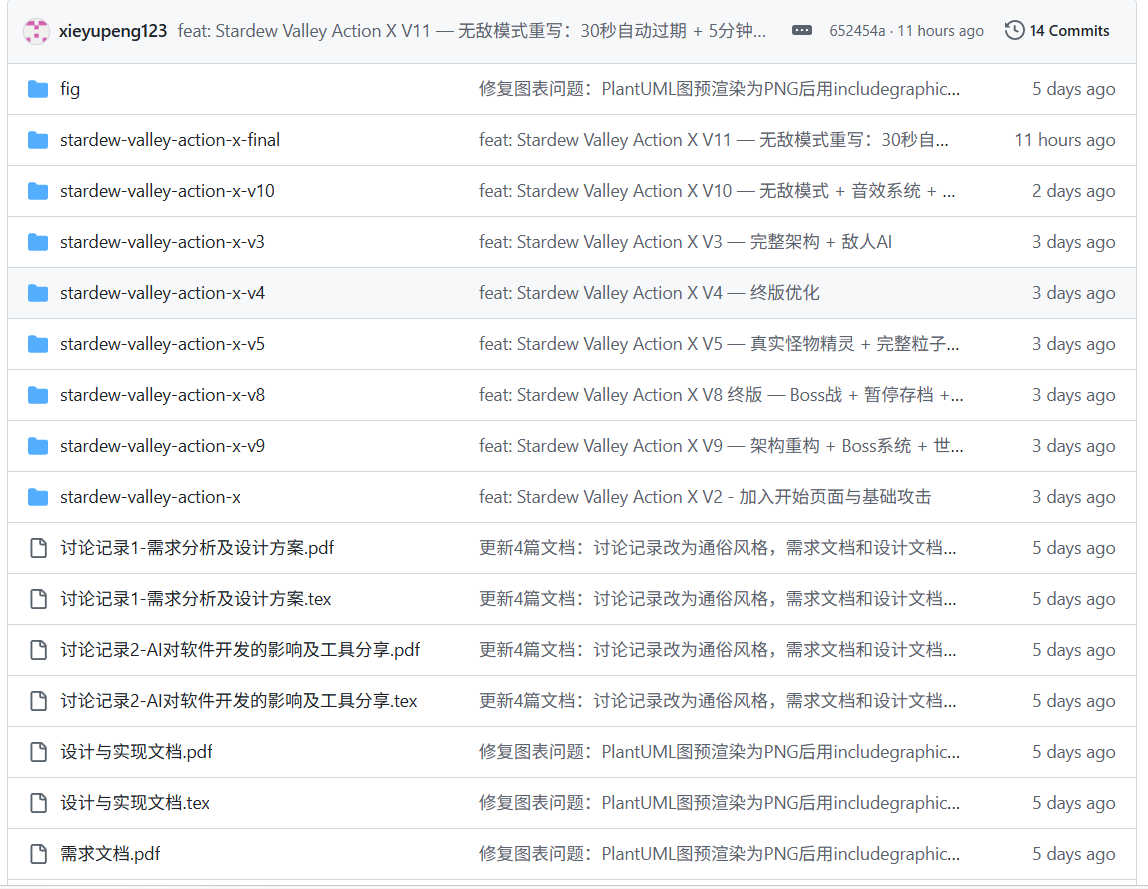
\includegraphics[width=\textwidth]{images/github/提交总览.png}
\caption{Git提交历史总览}
\label{fig:commit_overview}
\end{figure}

\begin{figure}[H]
\centering
\begin{minipage}[t]{0.49\textwidth}
\centering
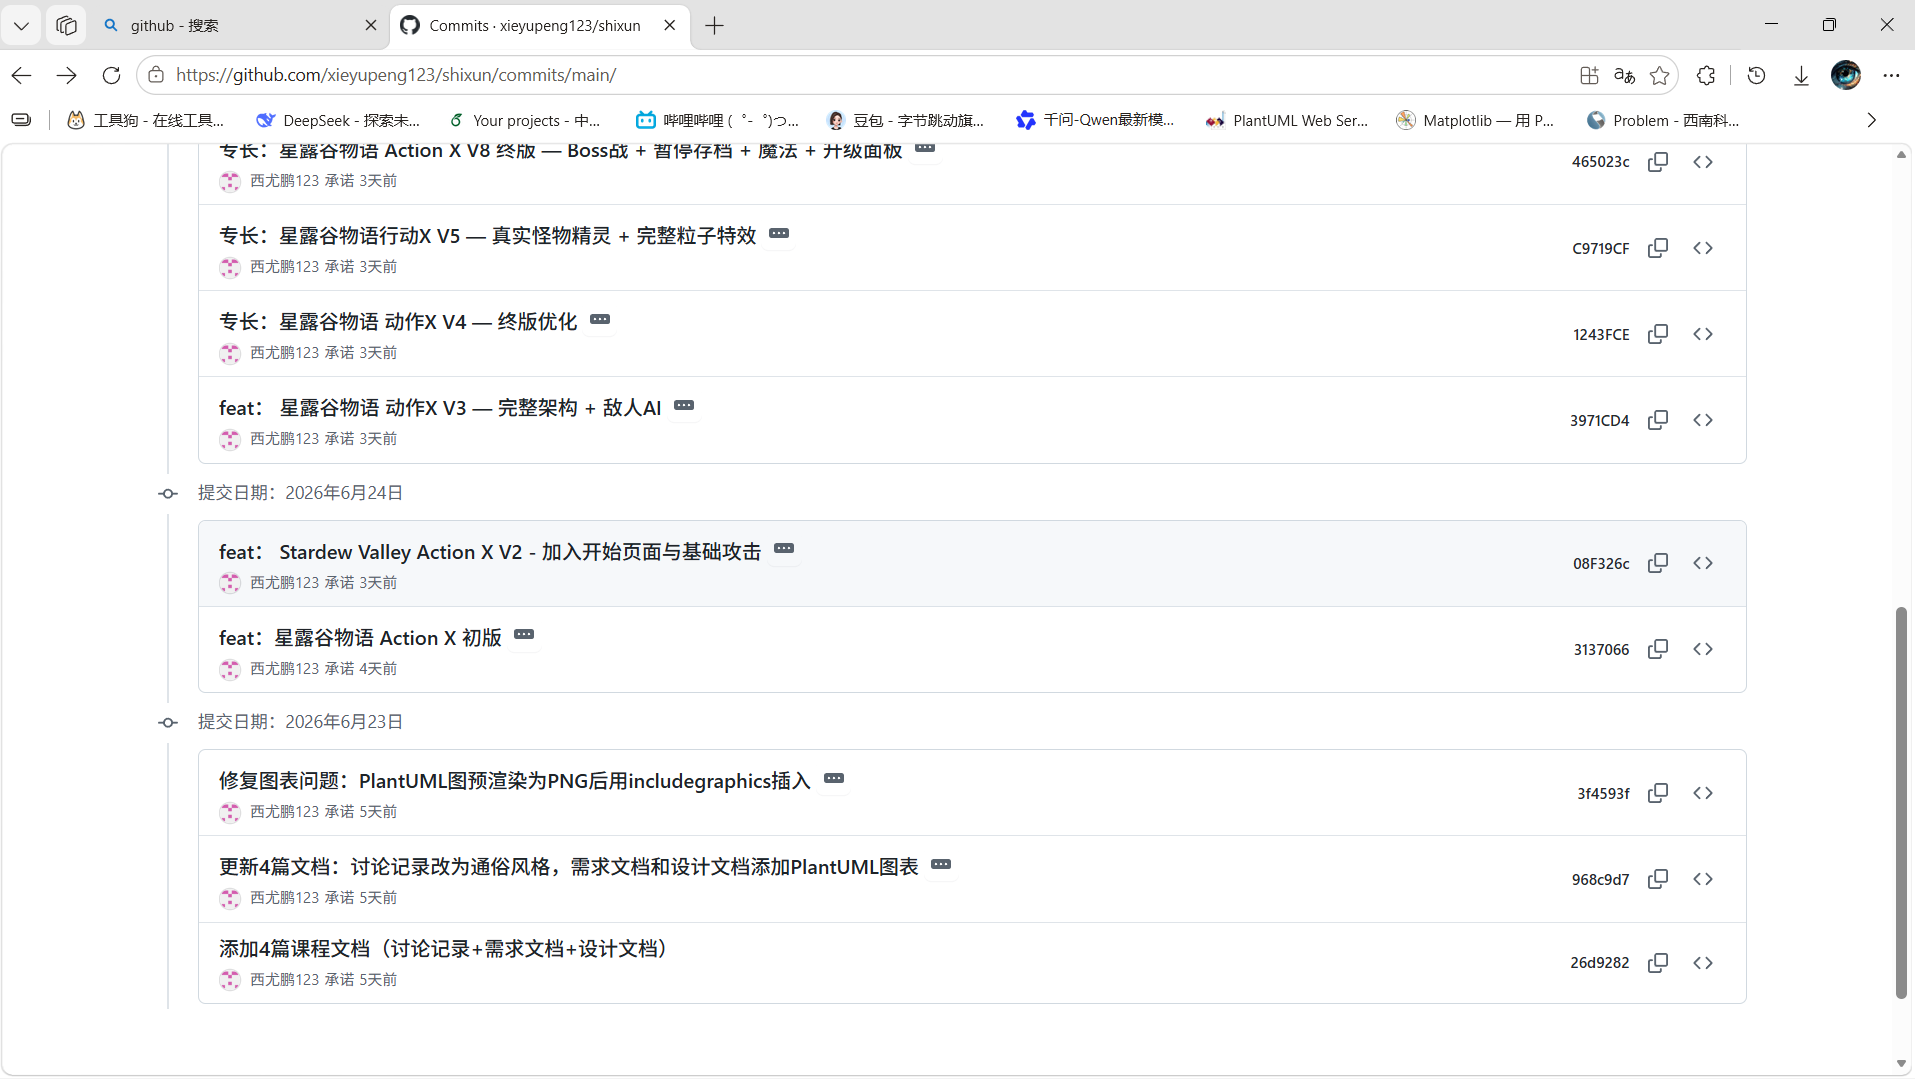
\includegraphics[width=\textwidth]{images/github/具体提交其一.png}
\caption{提交详情一：文档阶段与初版至V4}
\end{minipage}
\hfill
\begin{minipage}[t]{0.49\textwidth}
\centering
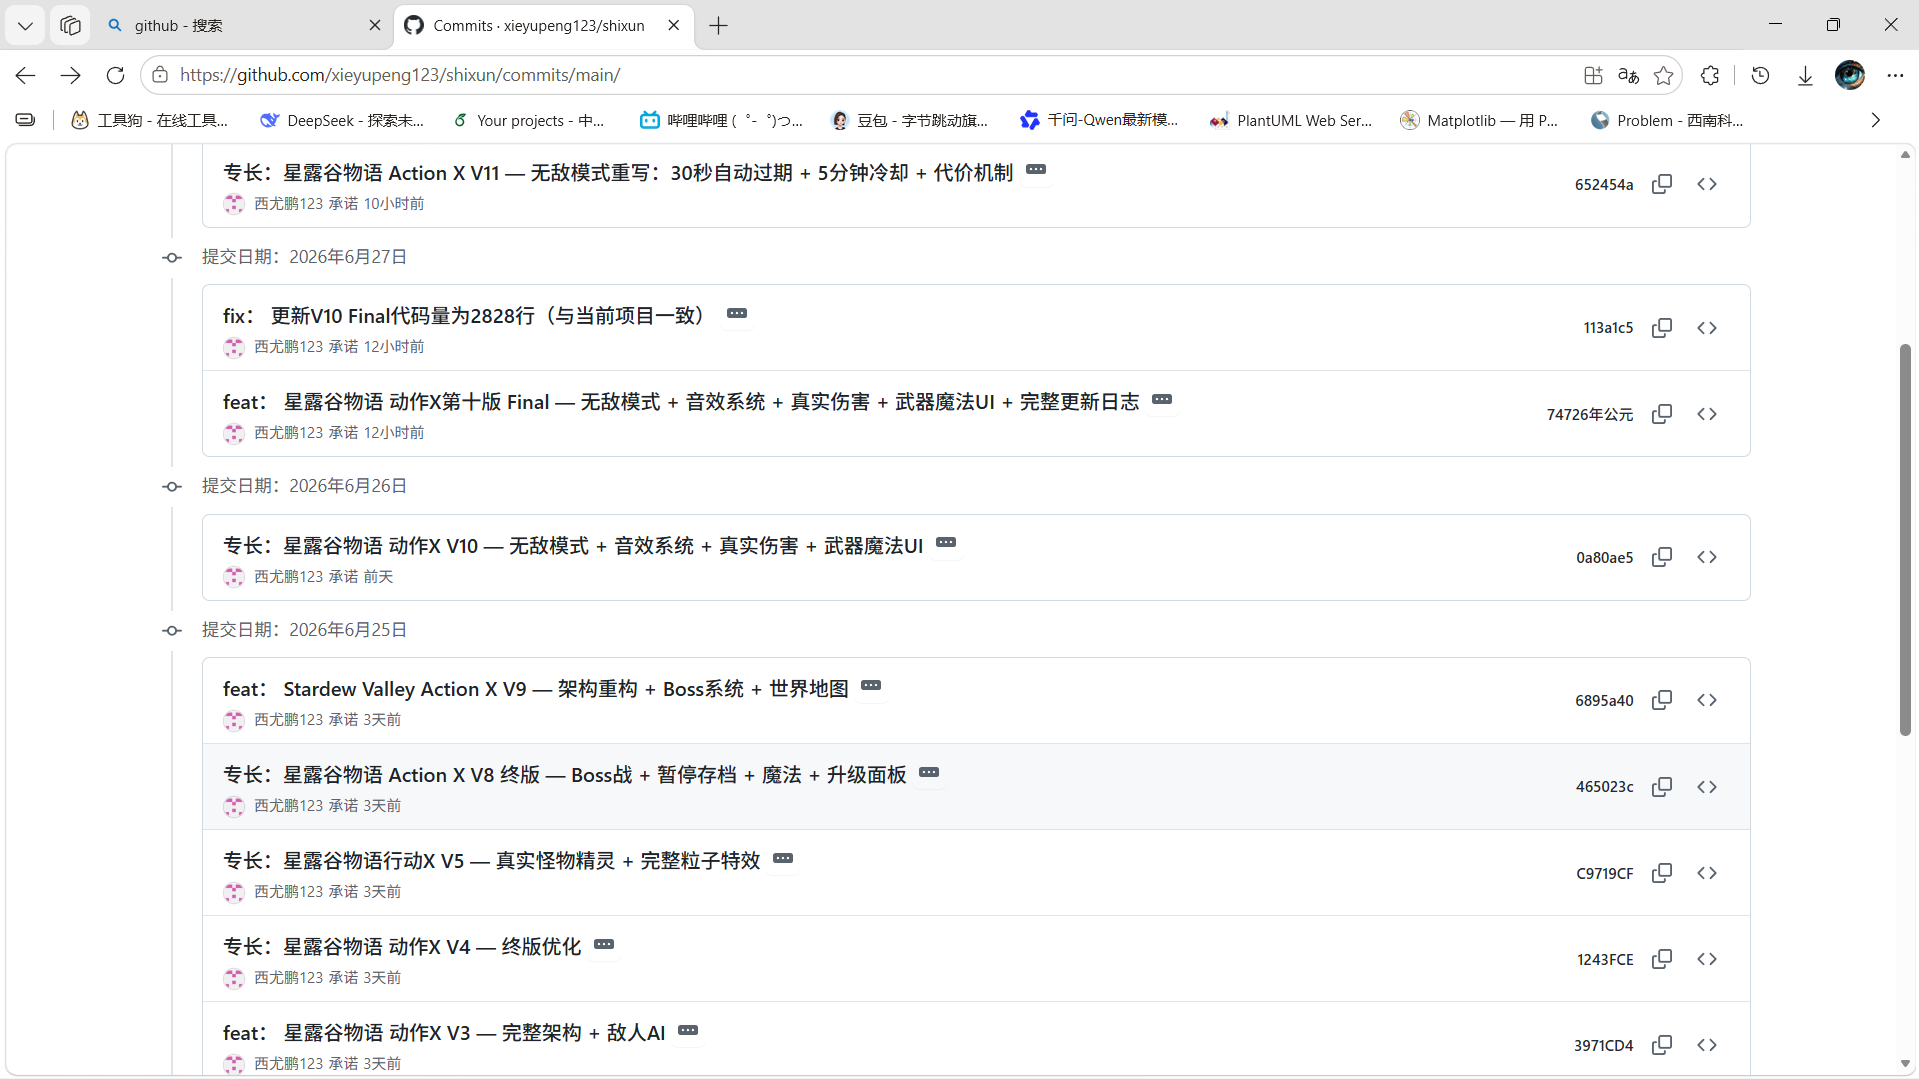
\includegraphics[width=\textwidth]{images/github/具体提交其二.png}
\caption{提交详情二：V5至V10版本}
\end{minipage}
\end{figure}

\begin{figure}[H]
\centering
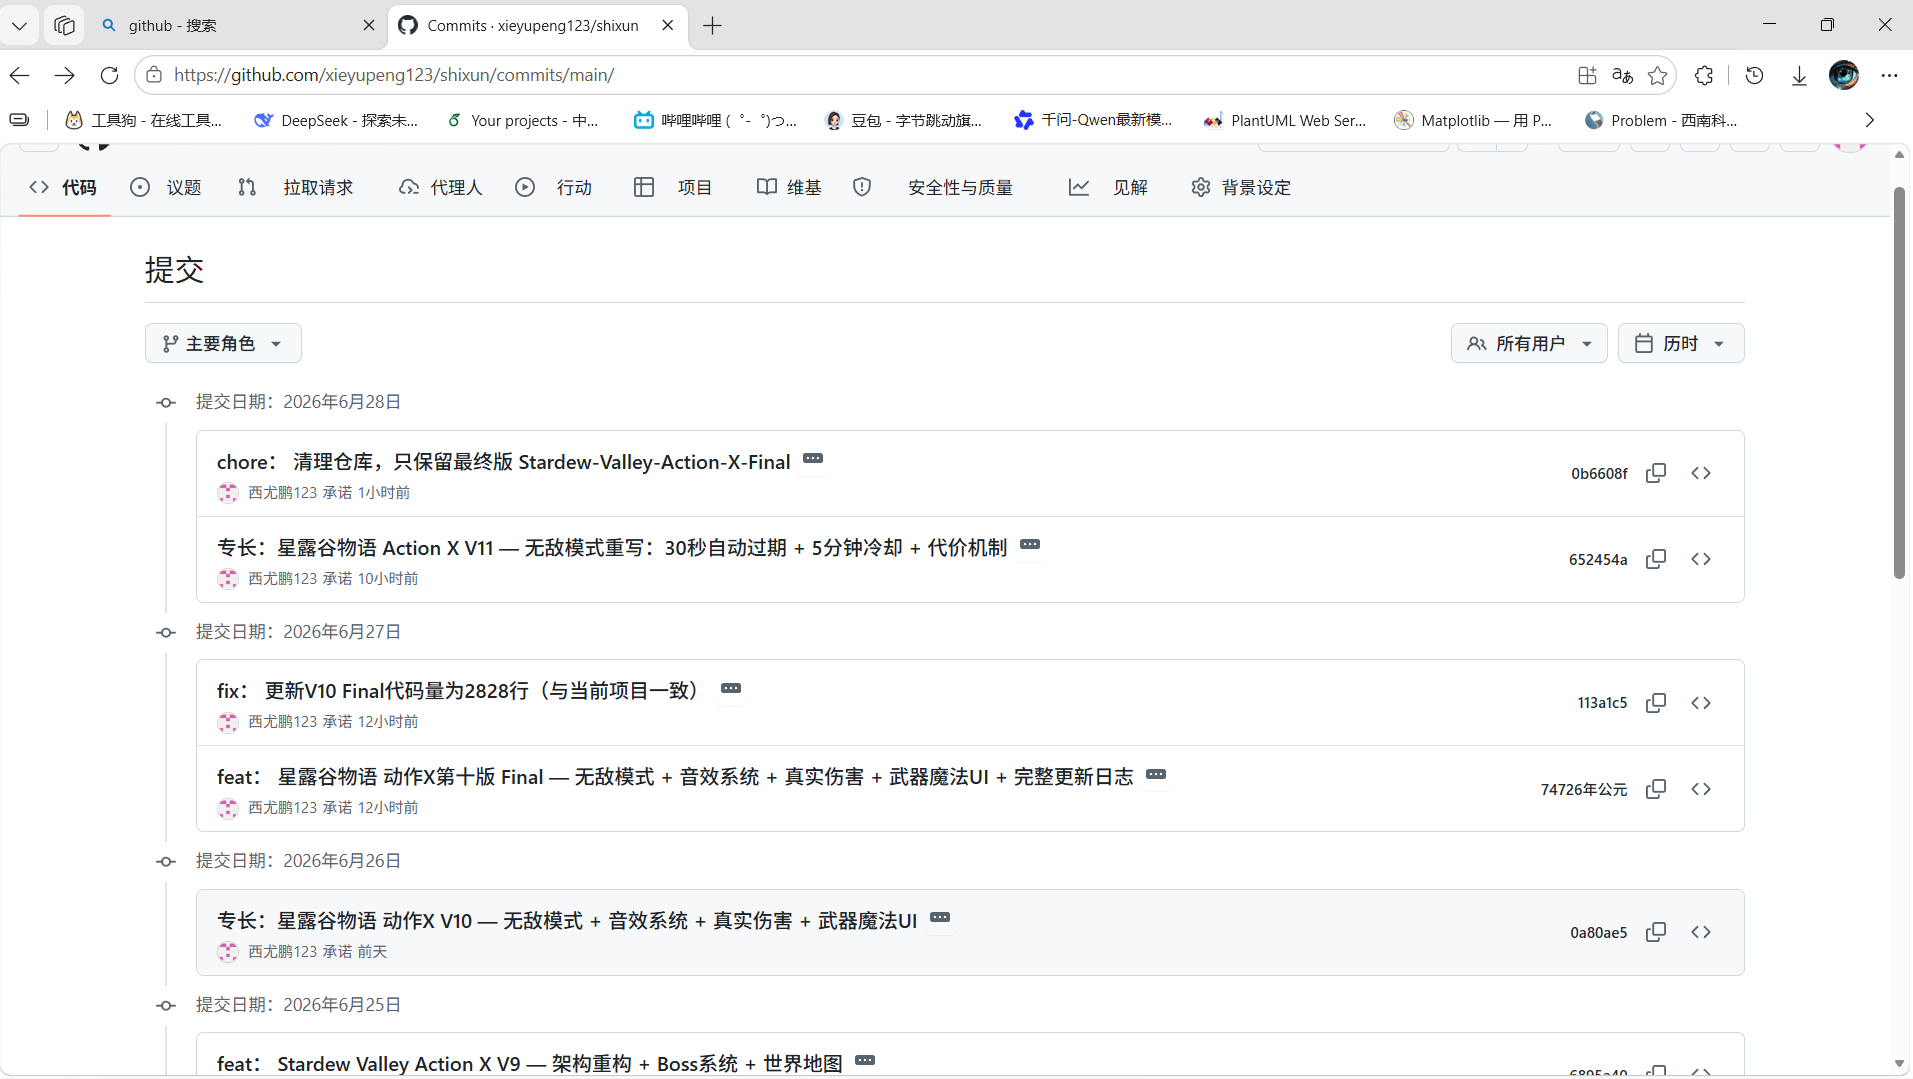
\includegraphics[width=0.85\textwidth]{images/github/具体提交其三.png}
\caption{提交详情三：V10 Final至V11完整版}
\label{fig:commit_detail3}
\end{figure}

\begin{table}[H]
\centering
\small
\begin{tabular}{>{\raggedright\arraybackslash}p{1.4cm}>{\raggedright\arraybackslash}p{1cm}>{\raggedright\arraybackslash}p{0.6cm}>{\raggedright\arraybackslash}p{9cm}}
\toprule
\textbf{日期} & \textbf{Hash} & \textbf{版本} & \textbf{提交说明} \\
\midrule
06/23 14:20 & 26d9282 & --- & 添加4篇课程文档（讨论记录+需求文档+设计文档） \\[3pt]
06/23 16:00 & 968c9d7 & --- & 更新4篇文档为通俗风格，添加PlantUML图表 \\[3pt]
06/23 16:16 & 3f4593f & --- & 修复PlantUML图预渲染为PNG后插入 \\[3pt]
06/24 17:03 & 3137066 & V1 & 初版：基础窗口和角色显示 \\[3pt]
06/24 23:46 & 08f326c & V2 & 加入主菜单页面与基础攻击系统 \\[3pt]
06/25 08:19 & 3971cd4 & V3 & 完整四层分层架构 + 敌人AI状态机 \\[3pt]
06/25 09:26 & 1243fce & V4 & 终版优化：代码重构与性能提升 \\[3pt]
06/25 10:43 & c9719cf & V5 & 真实怪物精灵 + 完整粒子特效系统 \\[3pt]
06/25 18:54 & 465023c & V8 & Boss战+暂停存档+魔法释放+升级面板 \\[3pt]
06/25 23:12 & 6895a40 & V9 & 架构重构：组合模式 + Boss三阶段 + 世界地图 \\[3pt]
06/26 08:17 & 0a80ae5 & V10 & 无敌模式+音效系统+真实伤害+武器魔法UI \\[3pt]
06/27 22:27 & 74726ad & V10F & V10 Final：完整更新日志 \\[3pt]
06/27 22:34 & 113a1c5 & --- & 更新V10 Final代码量为2828行 \\[3pt]
06/28 00:33 & 652454a & V11 & 无敌模式重写：30秒自动过期+5分钟冷却+代价机制 \\[3pt]
06/28 11:43 & 1754d54 & --- & 添加提示词文档集合（系统提示词+各阶段开发指南） \\
\bottomrule
\end{tabular}
\caption{项目完整提交历史详表}
\label{tab:commits}
\end{table}

\subsection{版本控制反思}

在本次项目中，我采用的版本控制策略可以概括为\textbf{「架构优先，增量迭代，大版本突变提交，本地同步备份」}：

\begin{enumerate}[label=(\arabic*)]
    \item \textbf{架构优先，增量迭代}。以V3为里程碑，首先建立四层分层架构的骨架。后续版本在此骨架上增量添加功能：V4优化、V5添加美术资源、V8引入Boss和升级系统、V9架构重构。每次改动都确保在已有架构框架内进行。

    \item \textbf{工作粒度与功能完整度匹配}。每个提交对应一个明确的功能里程碑：V8一次性引入Boss战、暂停存档、魔法、升级面板四个系统，粒度虽大但功能自成闭环；V4是纯代码优化，可以独立回溯。这种策略使每次提交都具有独立的可运行性和可测试性。

    \item \textbf{本地同步备份，防范云端风险}。每次云端提交前确保本地通过测试验证。本地保有多份历史备份，为云端可能出现的误操作提供回旋余地。实践中确实遇到了远端仓库被清理的情况（提交0b6608f），得益于充分的本地备份，所有历史版本得以完整恢复，未造成数据损失。

    \item \textbf{持续集成的开发节奏}。提交跨越6天，每天集中开发并提交，实现了符合学生项目特点的持续开发节奏。
\end{enumerate}

%============================================
% CHAPTER 2
%============================================

\section{AI协作能力专项测评}

\subsection{与AI结对编程——调试/功能实现实录}

\subsubsection{(1) 问题描述}

在游戏开发中，我所遭遇的最棘手的技术难点是\textbf{多重BGM的切换循环冲突和覆写问题}。该问题本质上是一个全局状态一致性问题：系统同时维护普通BGM、Boss BGM、无敌音效三套音效通道，而切换逻辑散布在Player、Level、Game等多个模块中，缺乏统一的互斥保护。

我将问题归纳为以下五个典型场景：

\begin{table}[H]
\centering
\small
\begin{tabularx}{\textwidth}{>{\raggedright\arraybackslash}p{1cm}>{\raggedright\arraybackslash}p{3.8cm}>{\raggedright\arraybackslash}p{3.2cm}>{\raggedright\arraybackslash}p{4.2cm}}
\toprule
\textbf{场景} & \textbf{触发条件} & \textbf{表现} & \textbf{根因} \\
\midrule
1 & Boss击杀后调用\_restart\_game()，MusicState仍为1 & 普通地图播放Boss战斗音乐 & \_restart\_game()遗漏了MusicState.reset()调用 \\[6pt]
2 & 普通BGM下激活无敌→进入Boss区域(MusicState$\rightarrow$1)→无敌到期 & BGM未切换到Boss音乐，恢复了普通BGM & \_end\_invincibility()的路径判断逻辑有缺陷 \\[6pt]
3 & 无敌状态下冲入Boss区域→无敌到期 & 所有音效完全丢失，游戏无声 & 多个pygame.mixer.music操作缺乏互斥保护 \\[6pt]
4 & Boss BGM触发条件错误：必须受到Boss攻击才切换 & 即使已靠近Boss，只要未受击就保持普通BGM & 触发逻辑使用了攻击事件而非A*寻路的探测范围 \\[6pt]
5 & BGM已切为Boss音乐后，后台每帧仍在轮询检测距离 & Boss战期间持续无效运算，造成CPU浪费 & 缺少\"已触发则跳过\"的短路判断机制 \\
\bottomrule
\end{tabularx}
\caption{BGM多层切换问题的五个典型场景}
\end{table}

问题的核心在于BGM功能涉及多重变化和时机切换，而切换逻辑各自为政，没有统一的状态管理器。这类似于操作系统中\textbf{多个进程同时操作共享变量而没有引入互斥锁}导致的竞态条件问题。此外，BGM触发条件和轮询效率也存在设计缺陷，整体形成了一个多层次、彼此交织的复杂问题网络。

\begin{figure}[H]
\centering
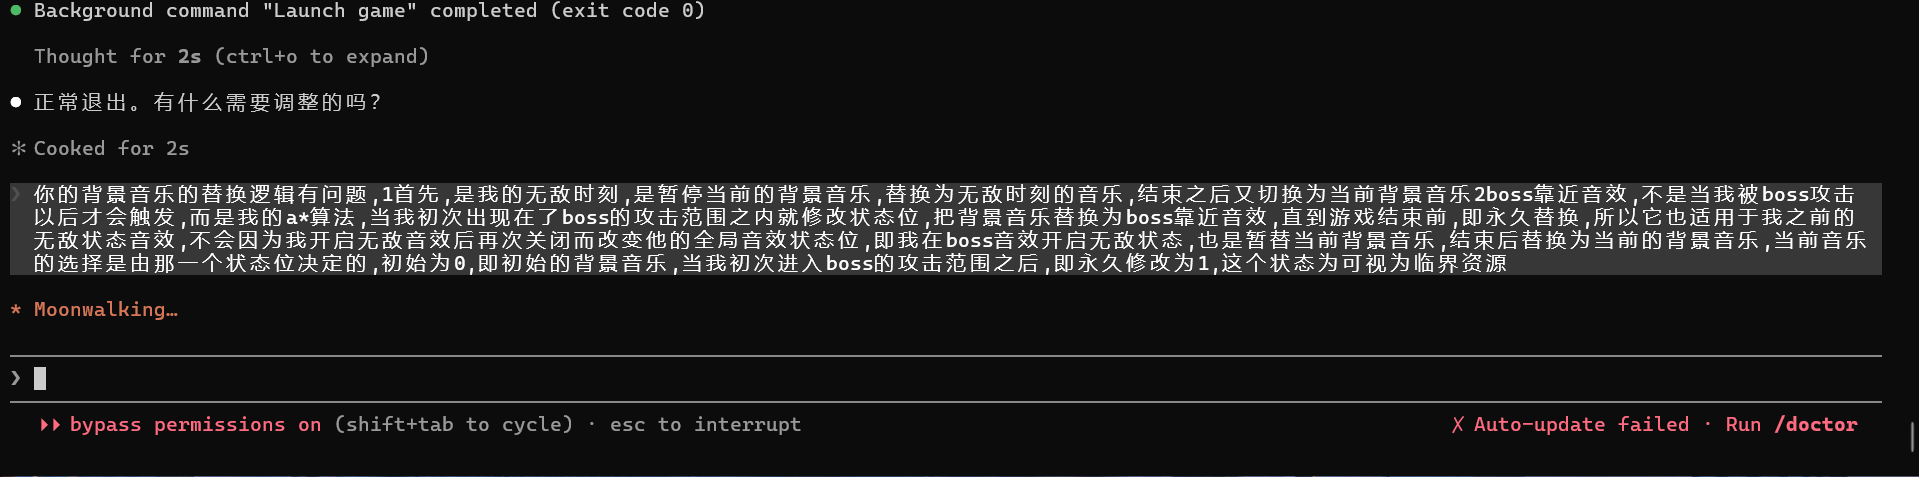
\includegraphics[width=0.85\textwidth]{images/github/提供整体的bgm设计方案和临界资源锁定问题.png}
\caption{向AI描述BGM设计方案和临界资源锁定问题}
\label{fig:bgm_prompt}
\end{figure}

\subsubsection{(2) 你的AI提示词}

以下为调试过程中输入给AI的关键Prompt内容：

\begin{quote}\small
「我现在遇到了BGM多层切换引起的音效混乱问题。项目背景：普通地图播放game\_bgm.ogg；进入Boss区域后自动切换到boss\_bgm.ogg；按空格激活无敌模式时停止当前BGM并循环播放invincible.ogg。

我发现了五个问题：（1）Boss被击杀后重启游戏，普通地图仍在播放Boss音乐，请检查\_restart\_game()中MusicState.reset()是否被调用；（2）无敌→进入Boss区域→无敌到期，BGM切回了普通音乐而非Boss音乐，\_end\_invincibility()的路径判断有缺陷；（3）无敌状态挑战Boss→无敌到期后所有音效丢失，怀疑pygame.mixer操作之间缺少互斥保护；（4）Boss BGM触发条件当前是受到攻击才切换，应该改为进入A*notice\_radius就触发；（5）BGM已经切为Boss音乐后，后台还在每帧轮询距离检测，造成CPU浪费，需要加入短路判断。

请参考操作系统的\textbf{信号量机制和互斥思想}来重新设计BGM管理方案。要求：每次重启先重置状态量；BGM加载必须通过MusicState的get()/set()/reset()三个原语中转；无敌模式只能激活不能手动关闭；首次检测到进入范围即永久锁定状态直到游戏重启。请给出具体代码修改方案。」
\end{quote}

同时，我提供了带有时间戳的运行日志截图，帮助AI理解具体的状态转换和错误位置：

\begin{figure}[H]
\centering
\begin{minipage}[t]{0.49\textwidth}
\centering
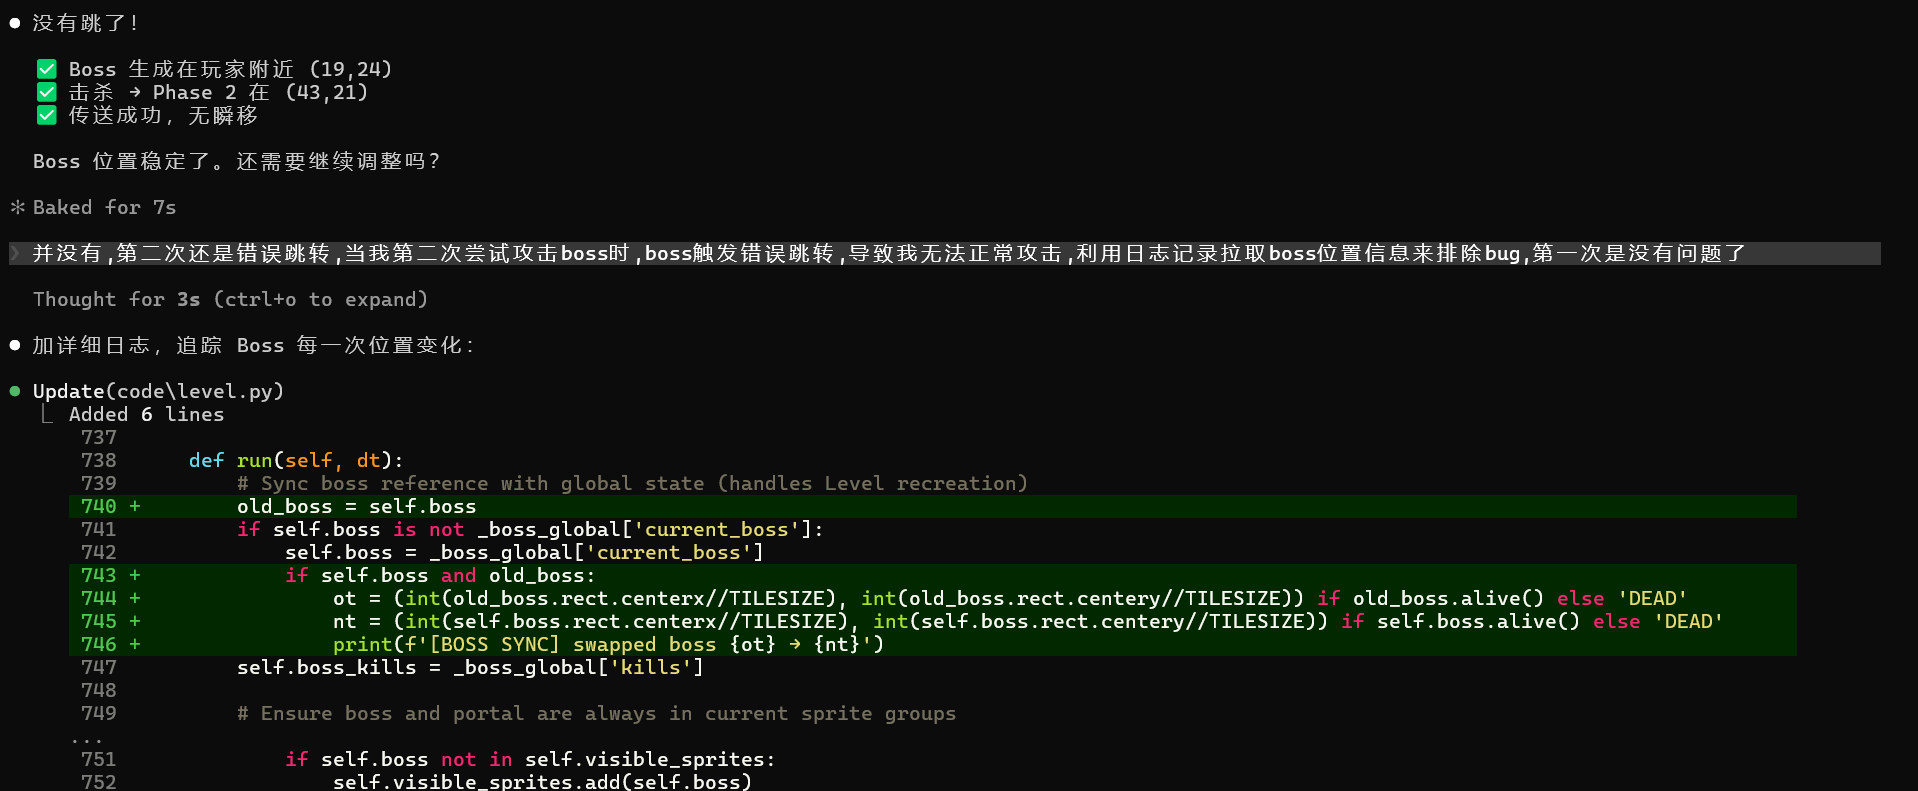
\includegraphics[width=\textwidth]{images/github/用日志拉取击败boss后的位置状态修复错误跳转的bug.png}
\caption{通过日志拉取调试BGM状态问题}
\end{minipage}
\hfill
\begin{minipage}[t]{0.49\textwidth}
\centering
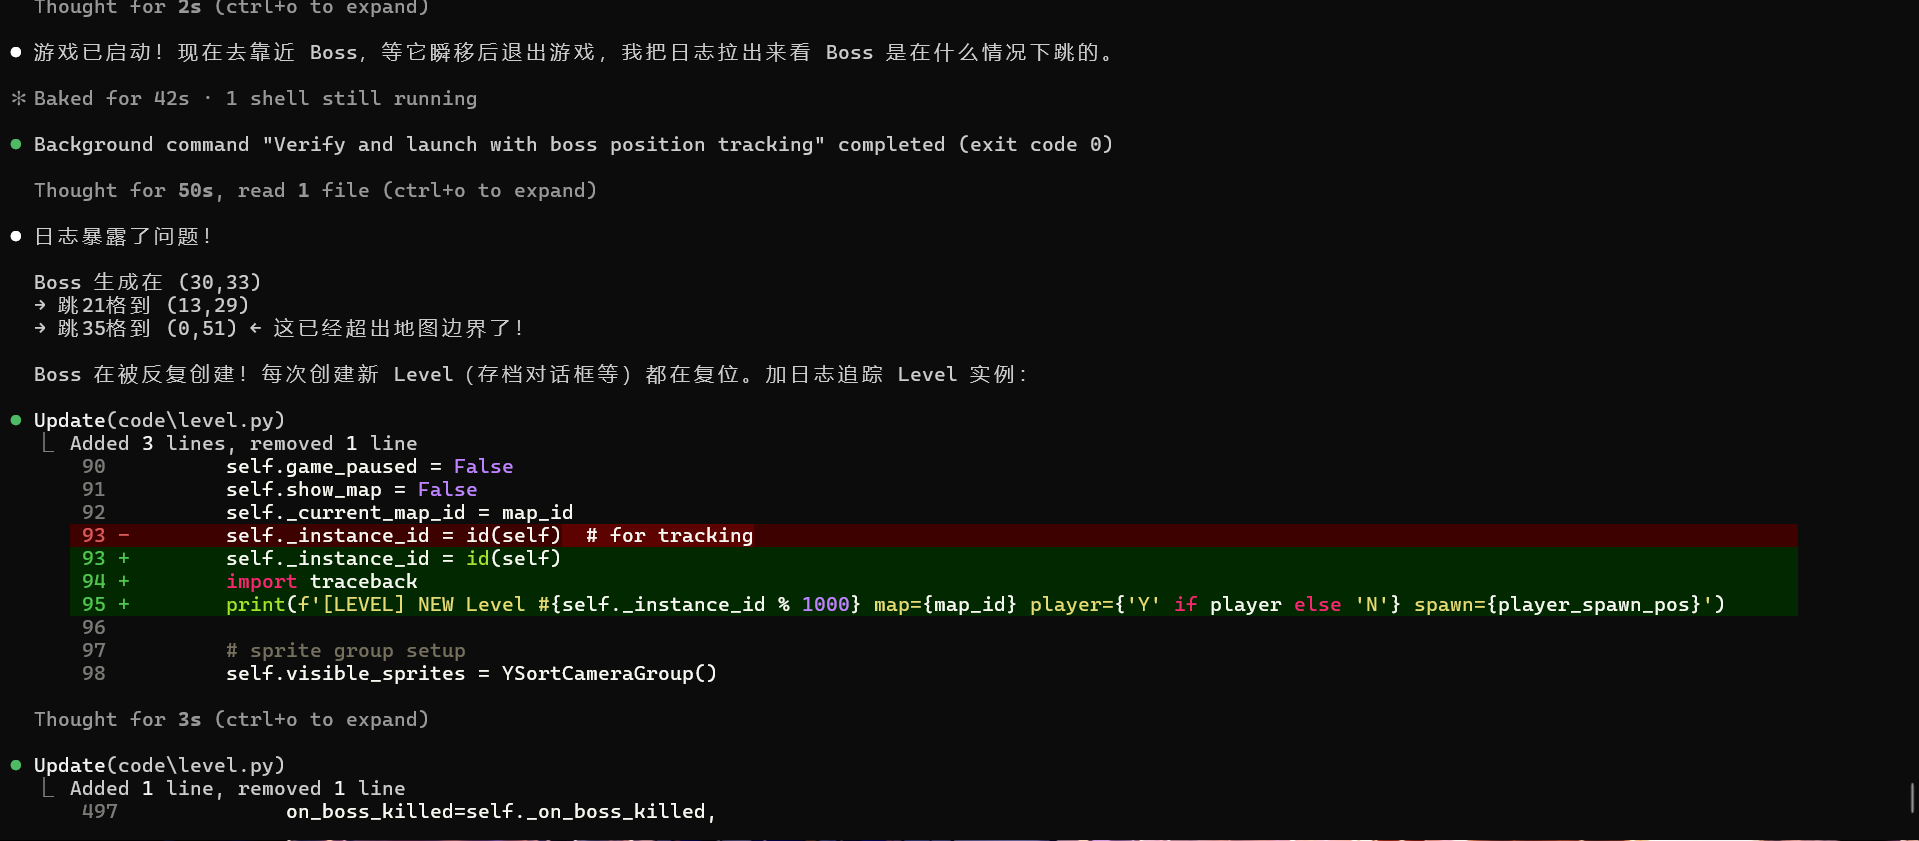
\includegraphics[width=\textwidth]{images/github/通过日志拉取成功解决问题.png}
\caption{日志分析后成功定位并修复BGM问题}
\end{minipage}
\end{figure}

\subsubsection{(3) AI给出的解决方案}

AI接收完整上下文后给出的初始方案如下（关键代码）：

\begin{lstlisting}[
    caption={AI初始方案的BGM恢复逻辑},
    label={lst:ai_bgm},
    basicstyle=\footnotesize\ttfamily
]
def _end_invincibility(self):
    self.invincible = False
    if self.invincible_sound:
        self.invincible_sound.stop()
    # ---- AI's problematic code ----
    if MusicState.get() == 1:
        # Check if channel is free before loading
        if not pygame.mixer.music.get_busy():
            pygame.mixer.music.load(get_path('../audio/boss_bgm.ogg'))
            pygame.mixer.music.set_volume(0.5)
            pygame.mixer.music.play(-1)
    else:
        pygame.mixer.music.load(get_path('../audio/game_bgm.ogg'))
        pygame.mixer.music.set_volume(0.3)
        pygame.mixer.music.play(-1)
\end{lstlisting}

\textbf{AI方案的致命缺陷}：在MusicState.get()==1的分支中增加了get\_busy()前置检查。当无敌音效正在循环播放时，get\_busy()返回true，代码跳过Boss BGM的加载——结果MusicState已是1但实际音频为空，系统进入无声死锁。AI没有意识到在多状态切换场景中，\textbf{检查当前播放状态不能替代加载正确目标音频}。

\subsubsection{(4) 你的最终处理方式}

\begin{center}
\fbox{\parbox{0.9\textwidth}{\centering\Large\bfseries C. AI的方案有缺陷，我指出了问题\\并让其修正，最终人机共同完成。}}
\end{center}

\vspace{0.5cm}

\textbf{选择理由与修正过程}：

我选择了选项C。AI的方案在大部分正常路径下是正确的，但在边界路径（无敌状态下进入Boss区域）存在由get\_busy()引发的死锁缺陷。经过分析，我提出了以下修正策略——五个修正点分别对应上述五个问题场景：

\begin{enumerate}[label=(\arabic*)]
    \item \textbf{每次\_restart\_game()先无条件调用MusicState.reset()}，清空所有残留状态后再启动新游戏。同时调用ResourceManager.instance().stop\_all\_sounds()和pygame.mixer.music.stop()清空音频通道（对应场景1）。
    \item \textbf{去掉\_end\_invincibility()中的get\_busy()死锁检查}，改为「先无条件停止，再按MusicState信号量决定加载目标BGM」，不依赖任何运行时状态判断（对应场景2和3）。
    \item \textbf{确立MusicState的三个原语为BGM唯一入口}，禁止任何模块直接操作pygame.mixer.music。这类似于操作系统中\textbf{信号量原语}的设计——所有对共享资源的访问必须通过统一的P/V操作（对应场景2和3）。
    \item \textbf{修改Boss BGM触发条件}——从「受到Boss攻击」改为「首次进入Boss的notice\_radius探测范围」。结合A*寻路算法中怪物的\texttt{notice\_radius}（Boss为400像素），在\texttt{\_check\_boss\_music()}中计算玩家与Boss的欧几里得距离，一旦距离小于探测半径即触发切换。Boss BGM设为与普通BGM同等的全局优先级，因此可以被无敌模式正常暂停和恢复（对应场景4）。
    \item \textbf{加入短路判断避免无效轮询}——在\texttt{\_check\_boss\_music()}方法顶部增加\texttt{if MusicState.get() == 1: return}。首次检测并切换后，后续所有帧的调用立即返回，不再执行距离计算。状态锁保持到\texttt{\_restart\_game()}调用\texttt{MusicState.reset()}才被清除，实现\textbf{「一次性检测，永久锁定」}（对应场景5）。
\end{enumerate}

以下是两个核心修正的最终代码：

\begin{lstlisting}[
    caption={Boss BGM检测与短路优化},
    label={lst:check_boss_music},
    basicstyle=\footnotesize\ttfamily
]
def _check_boss_music(self):
    """One-way switch: when player first enters boss notice
    radius (A* range), permanently switch to boss music."""
    # Short-circuit: already triggered, skip ALL checks
    if MusicState.get() == 1:
        return
    boss = self.boss.boss
    if boss and boss.alive():
        boss_vec = pygame.math.Vector2(boss.rect.center)
        player_vec = pygame.math.Vector2(self.player.rect.center)
        dist = (player_vec - boss_vec).magnitude()
        if dist <= boss.notice_radius:
            MusicState.set(1)
            if not self.player.invincible:
                pygame.mixer.music.stop()
                pygame.mixer.music.load(self._boss_bgm_path)
                pygame.mixer.music.set_volume(0.5)
                pygame.mixer.music.play(-1)
\end{lstlisting}

\begin{lstlisting}[
    caption={修正后的BGM恢复逻辑},
    label={lst:fixed_bgm},
    basicstyle=\footnotesize\ttfamily
]
def _end_invincibility(self):
    self.invincible = False
    self.invincible_start_time = None
    # Set 5-min cooldown
    self.invincible_cooldown_until = pygame.time.get_ticks() + INVINCIBLE_COOLDOWN
    # Cost: -50% current HP (min 1) + all energy drained
    self.health = max(1, int(self.health * (1 - INVINCIBLE_COST_HEALTH)))
    self.energy = 0
    # ---- FIXED: unconditionally stop, then load by semaphore ----
    if self.invincible_sound:
        self.invincible_sound.stop()
    if MusicState.get() == 1:
        bgm_path = get_path('../audio/boss_bgm.ogg'); vol = 0.5
    else:
        bgm_path = get_path('../audio/game_bgm.ogg'); vol = 0.3
    pygame.mixer.music.load(bgm_path)
    pygame.mixer.music.set_volume(vol)
    pygame.mixer.music.play(-1)
\end{lstlisting}

\textbf{在人机协作中学到的最重要一课}：

AI目前还很难彻底取代软件工程师。它的编码能力很强，但存在根本性的短板——\textbf{AI不会做概要设计，无法自主地从全局架构出发审视系统}。对于需求分析、概要设计、代码规范、架构设计，\textbf{这正是软件工程师立足于AI时代、让AI服务于我们的核心能力所在}。

AI时代开发的关键原则：\textbf{磨刀不误砍柴工}——前期的详细设计不会耽误进度，反而使最终方案与设计理念高度吻合。此外，\textbf{在AI改动文件之前必须本人亲自确认}每个修改的范围和影响，不能过于懒惰。

\subsubsection{多模态协作与API成本优化}

在本项目的AI协作中，我认为自己做得最好的方面是\textbf{多模型协作策略}。不同AI模型的API价格和能力各有侧重，我根据任务类型建立了分层使用策略：

\begin{table}[H]
\centering
\small
\begin{tabularx}{\textwidth}{>{\raggedright\arraybackslash}p{3cm}>{\raggedright\arraybackslash}p{2.8cm}>{\raggedright\arraybackslash}p{7.2cm}}
\toprule
\textbf{任务类型} & \textbf{选用模型} & \textbf{选择理由与应用场景} \\
\midrule
代码架构设计、Bug调试、逻辑推理 & DeepSeek V4 Pro & 推理能力世界一流，支持100万token上下文。用于BGM状态机修复、战斗系统设计、无敌模式逻辑等复杂任务 \\[4pt]
图像识别、地图构建、多模态分析 & MiMo V2.5/Pro & 具备图文识别能力，可分析PNG像素通道。用于水面蓝色通道检测、敌人精灵切图验证等视觉任务 \\[4pt]
简单读取、代码格式化、文档整理 & 基础模型/MiMo V2.5 & Token价格低廉，适合读取CSV地图文件、格式化注释、版本日志生成等轻量任务 \\
\bottomrule
\end{tabularx}
\caption{多模型分层协作策略}
\end{table}

此外，我编写了模型切换脚本（switch-model.ps1），只需一行命令即可切换模型并保留完整历史对话上下文，避免了手动修改配置文件导致对话丢失的问题。

\begin{figure}[H]
\centering
\begin{minipage}[t]{0.49\textwidth}
\centering
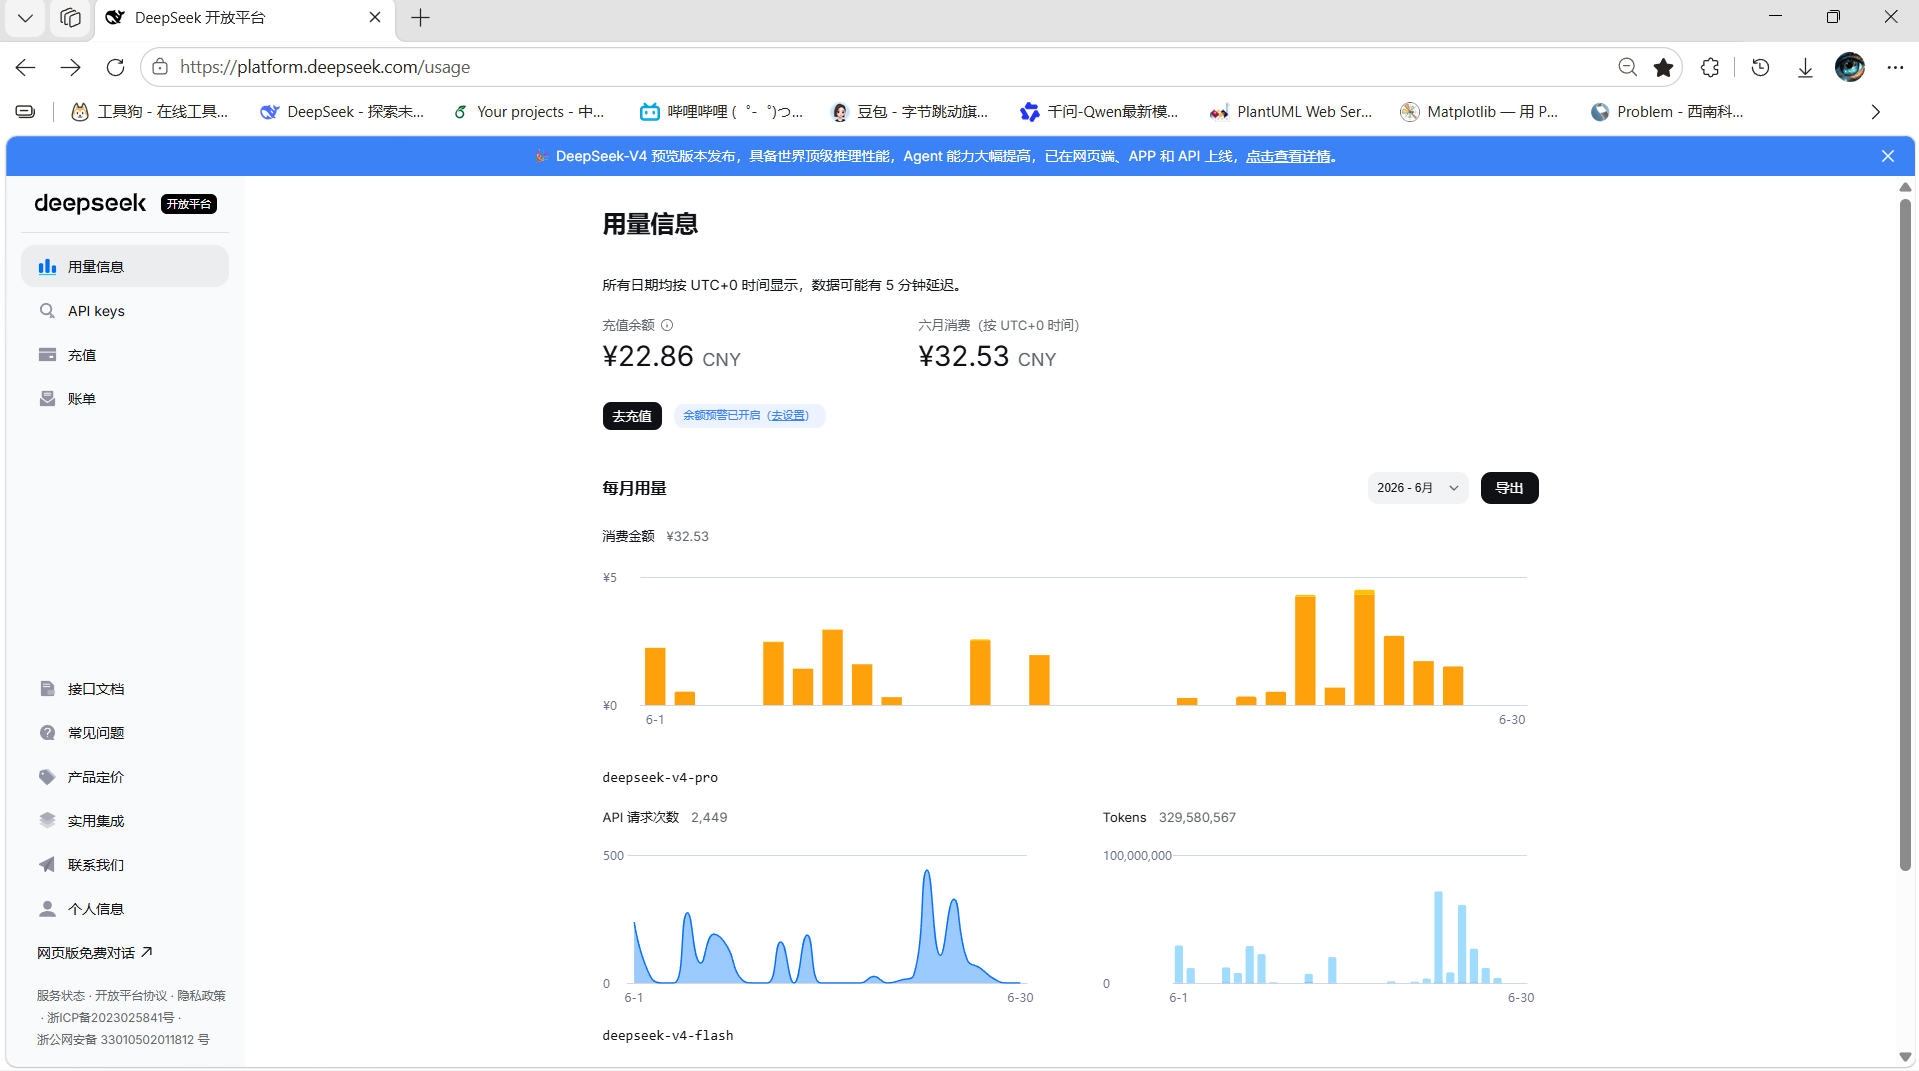
\includegraphics[width=\textwidth]{images/github/截止到周天deepseek_token消耗量_15RMb.png}
\caption{DeepSeek V4 Pro token消耗统计}
\end{minipage}
\hfill
\begin{minipage}[t]{0.49\textwidth}
\centering
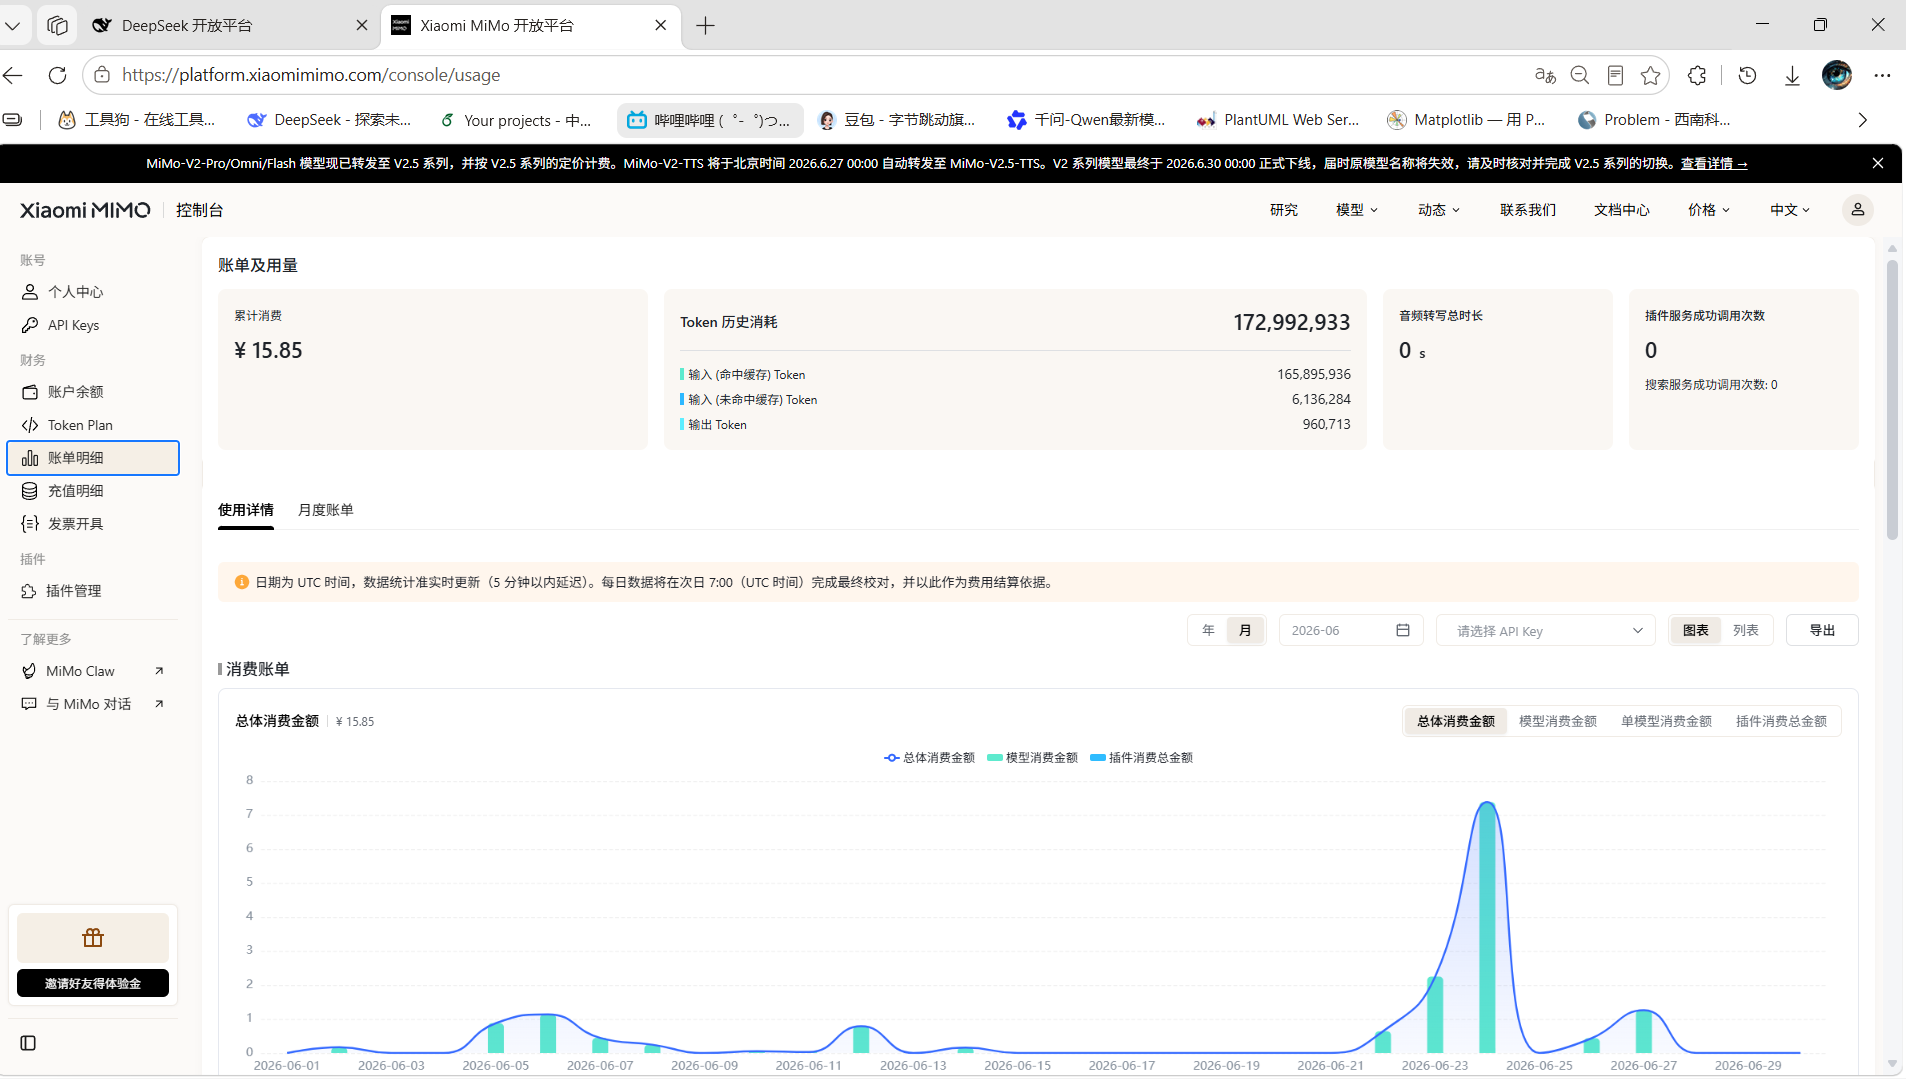
\includegraphics[width=\textwidth]{images/github/截至到周天mimo_token消耗量_11RMB.png}
\caption{MiMo系列token消耗统计}
\end{minipage}
\end{figure}

整个项目的AI协作总花费约26 RMB（DeepSeek约15 RMB + MiMo约11 RMB），在控制成本的同时实现了高质量的多模型协作。

%============================================
% CHAPTER 3
%============================================

\section{架构优化}

在项目的实际开发中，我对系统架构进行了从V1-V8（原始架构）到V9-V11（优化架构）的大幅优化。核心优化方向是：通过引入\textbf{组合模式}和\textbf{单例模式}，遵循\textbf{单一职责原则}和\textbf{分层架构原则}，将Level从「上帝类」重构为「协调者」。

\subsection{优化前架构}

\begin{figure}[H]
\centering
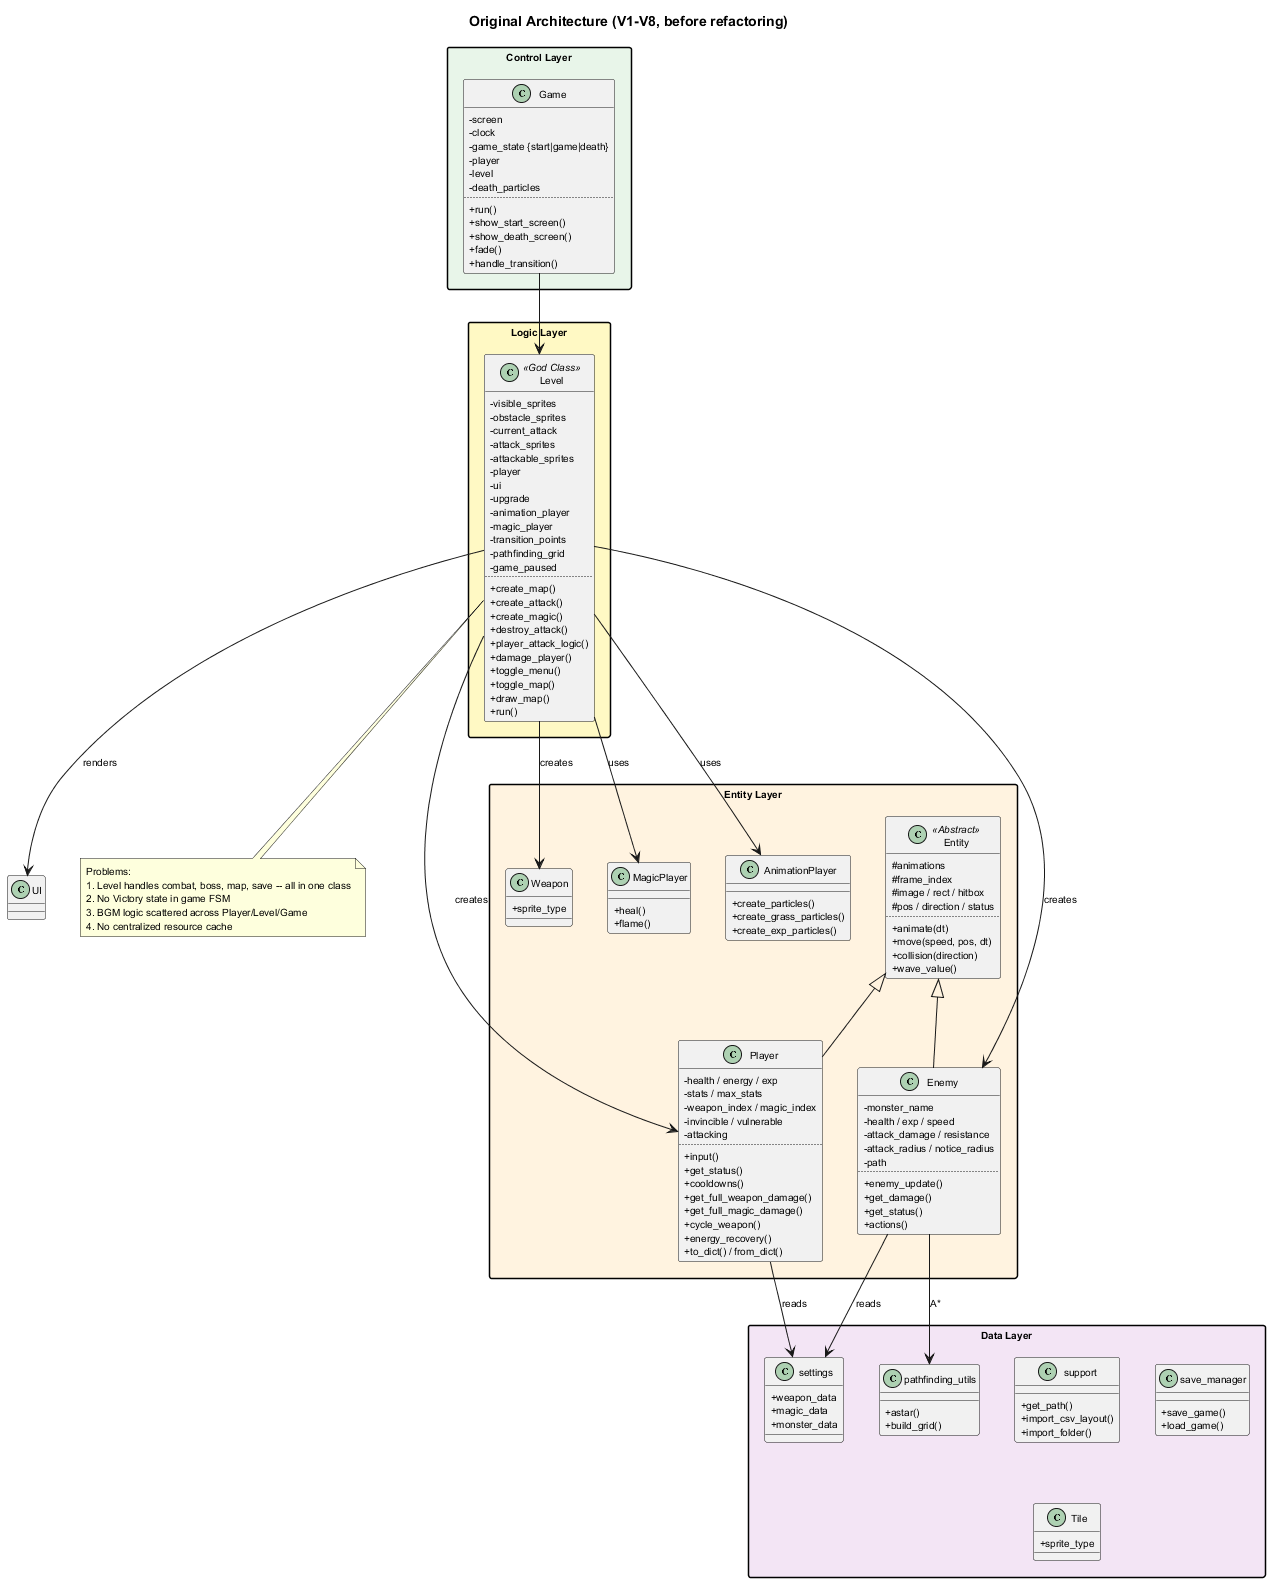
\includegraphics[width=\textwidth]{images/original_class_diagram.png}
\caption{系统优化前概要类图}
\label{fig:original_class}
\end{figure}

原始架构的核心问题：
\begin{enumerate}[label=\textbf{问题\arabic*：}, leftmargin=*]
    \item \textbf{Level为God Class（500+行）}——战斗逻辑、Boss管理、地图渲染、实体创建、传送检测、存档序列化全部堆在一个类中，违反SRP原则。任何功能修改都需要触碰这个巨型类。
    \item \textbf{缺少统一资源管理}——图片、音效、字体各自独立加载，同一文件可能被多次加载造成内存浪费。加载失败没有统一降级机制。
    \item \textbf{BGM状态管理缺失}——切换逻辑散布在Player、Level、Game三个模块中，各自直接操作pygame.mixer，导致竞态条件和状态不一致。
    \item \textbf{状态机不完整}——仅有start/game/death三种状态，缺少Victory结算界面。
\end{enumerate}

\subsection{优化后架构}

\begin{figure}[H]
\centering
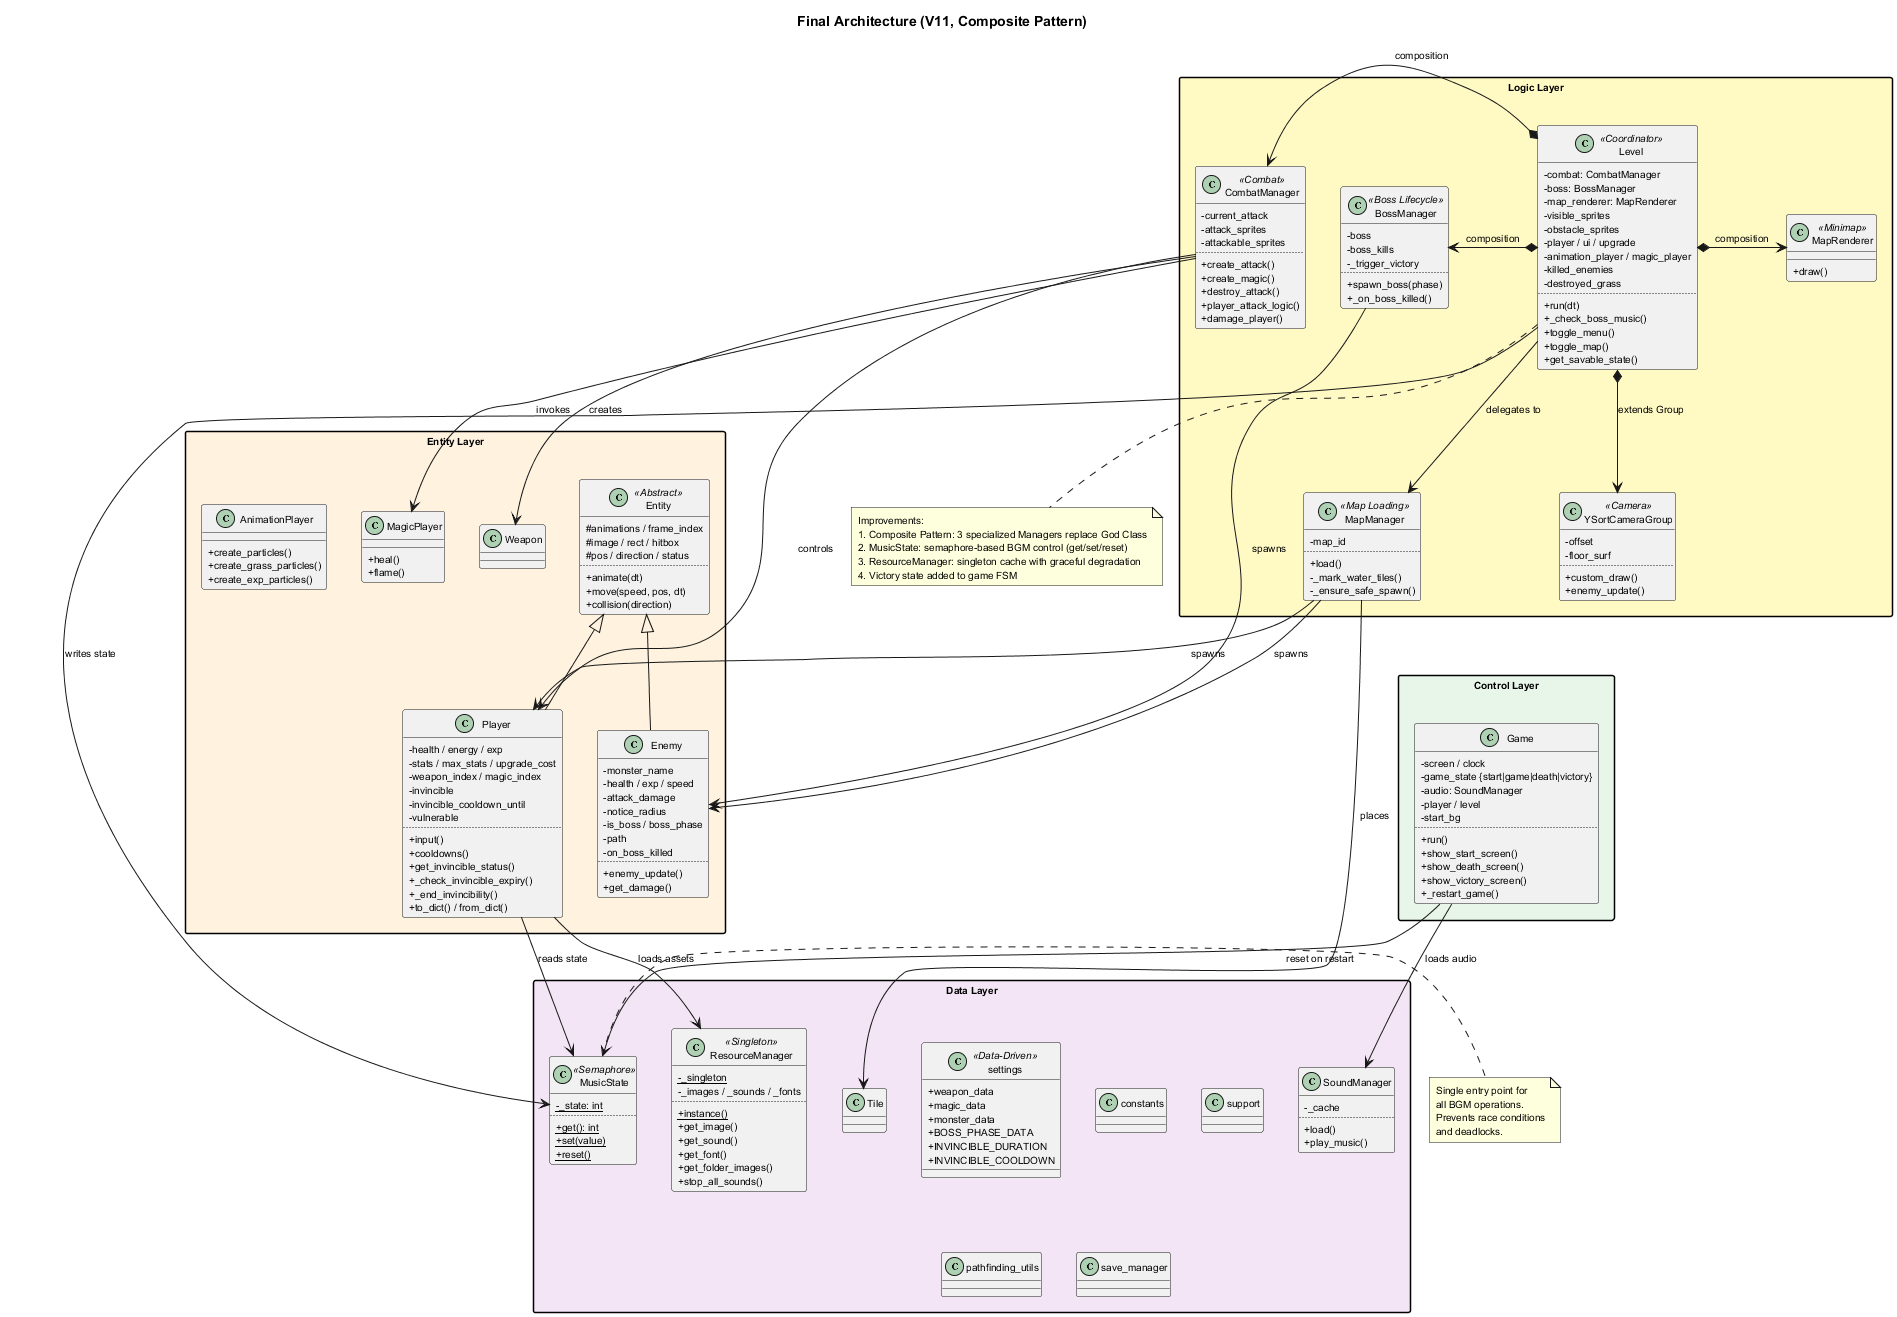
\includegraphics[width=\textwidth]{images/final_class_diagram.png}
\caption{系统优化后概要类图}
\label{fig:final_class}
\end{figure}

优化后的关键改进：
\begin{enumerate}[label=\textbf{优化\arabic*：}, leftmargin=*]
    \item \textbf{引入组合模式}——将Level拆分为CombatManager（战斗调度，约80行）、BossManager（Boss生命周期，约60行）、MapRenderer（地图叠加层，约100行）三个专职Manager，Level通过@property代理保持向下兼容。
    \item \textbf{引入MusicState单例（信号量机制）}——所有BGM操作统一经过get()/set()/reset()三个原语，禁止直接操作pygame.mixer，从根本上解决多层切换的死锁和丢失问题。
    \item \textbf{引入ResourceManager单例模式}——全局唯一资源缓存实例，图片/音效/字体统一管理、按路径缓存、失败静默降级。
    \item \textbf{新增Victory状态}——游戏状态机完整覆盖start→game→(death | victory)的全生命周期。
    \item \textbf{引入MapManager}——将CSV地图加载、四层瓦片铺设、水域像素检测、寻路网格构建全部封装为独立类，并实现水域检测结果缓存。
\end{enumerate}

\subsection{BGM状态机设计}

\begin{figure}[H]
\centering
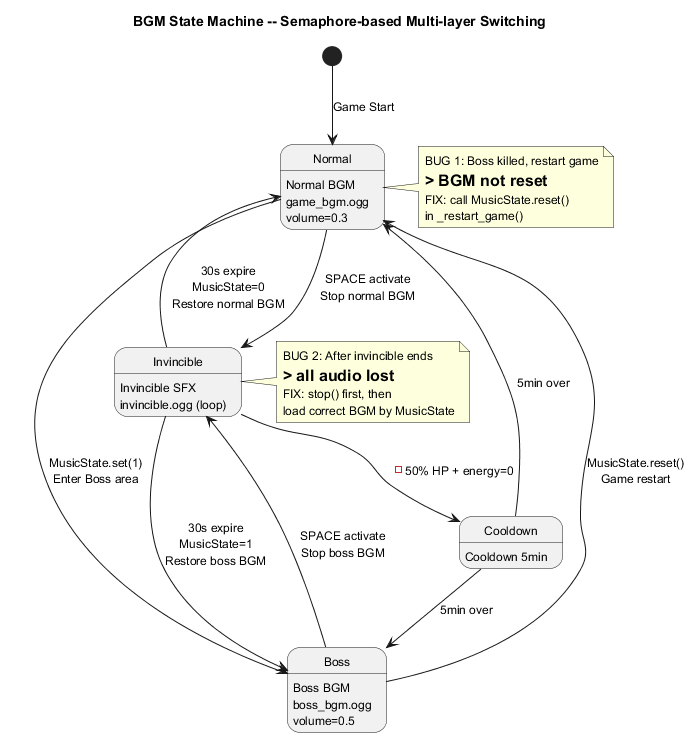
\includegraphics[width=0.75\textwidth]{images/bgm_fsm.png}
\caption{BGM状态机}
\label{fig:bgm_fsm}
\end{figure}

该状态机的设计灵感来源于操作系统中的\textbf{信号量}概念：MusicState作为一个二值信号量（0/1），所有BGM消费者必须通过统一原语读写状态，且reset()操作在任何重启路径上始终被保证执行。通过这种方式，MusicState的内部值与pygame.mixer.music的实际播放内容始终保持一致。

\subsection{设计原则与设计模式}

\begin{table}[H]
\centering
\small
\begin{tabularx}{\textwidth}{>{\raggedright\arraybackslash}p{2.8cm}>{\raggedright\arraybackslash}p{5.2cm}>{\raggedright\arraybackslash}p{5.2cm}}
\toprule
\textbf{原则/模式} & \textbf{在本项目中的具体体现} & \textbf{带来的收益} \\
\midrule
单一职责原则 & Level拆分为CombatManager、BossManager、MapRenderer & 每个类只有一条需要变更的理由，修改独立 \\[4pt]
组合模式 & Level通过组合引用集成各Manager，而非继承 & 新增功能域只需新建Manager并组合，无需修改已有代码 \\[4pt]
单例模式 & ResourceManager和MusicState各只有一个全局实例 & 资源缓存统一、BGM状态全局唯一 \\[4pt]
开闭原则 & 武器/怪物/魔法属性集中在settings.py字典中 & 新增类型只需加配置，不需改核心逻辑 \\[4pt]
分层架构 & 控制层→逻辑层→实体层→数据层，单向依赖 & 依赖方向可控，便于独立测试和替换底层 \\[4pt]
数据驱动设计 & 所有游戏数值集中于settings.py配置文件 & 策划调整数值无需开发者介入；配置即文档 \\
\bottomrule
\end{tabularx}
\caption{架构优化采用的设计原则和设计模式}
\end{table}

我的代码架构几乎在项目一开始（V3阶段）就确定好了四层分层结构，后续的音乐环节只引入了几个额外类（MusicState、SoundManager），在保持核心架构不变的前提下优化了耦合度。这与软件工程中「架构先行、迭代优化」的理念一致——核心架构在前期设计时敲定，之后的每次迭代都在稳固的框架下进行增量优化。

\end{document}
